\chapter[Referências]{Referências}

\section{Aprendizado Infantil}

As crianças passam pelo processo de desenvolvimento e de aprendizagem, muita das vezes estes conceitos são confundidos
entre si. O desenvolvimento de uma criança é um processo espontâneo, neste âmbito tem-se o desenvolvimento do corpo, do
sistema nervoso, e das funções mentais. O desenvolvimento está relacionado a todas as estruturas do conhecimento. Por
outro lado a aprendizagem não é um processo espontâneo, pelo contrário é um processo forçado, localizado apenas em um
dos âmbitos do desenvolvimento \cite{piaget:1972}.

Segundo a psicóloga Tharrany de Queiroz Silveira, as crianças começam a desenvolver o raciocínio lógico aproximadamente
entre 7 e 12 anos. Mas isso depende do desenvolvimento de cada criança. Esta fase em que começam a desenvolver o
raciocínio lógico coincide também com a idade que a criança inicia o ensino fundamental. Porém cabe ressaltar que com
os estímulos pelas quais as crianças, desde muito pequenas são expostas tornam seu desenvolvimento cognitivo cada vez
mais precoce e acelerado. As crianças são estimuladas pelo que é tátil, auditivo e visual. Como elas estão no mundo do
concreto, gostam de pegar interagir com o mundo externo.

A aprendizagem é muito mais eficaz quando se inclui a ludicidade, pois entendemos que a linguagem da criança, desde as
fases iniciais, ainda basicamente motora, é a brincadeira. Utilizar destes recursos para incentivar a aprendizagem,
auxilia as crianças, promovendo o desenvolvimento cognitivo. Quando optamos por utilizar da
tecnologia encontramos motivação para aprendizagem, visto que hoje a criança é inserida neste contexto cada vez mais
cedo: basta dar um celular pra criança ainda no primeiro ano de vida que rapidamente ela imita o movimento dos adultos
nas telas de touchscreen [de Queiroz Silveira 2015].

Mais especificamente, o desenvolvimento de uma criança está dividido em quatro estágios. Cada estágio corresponde a um
período do pensamento e do comportamento da criança. Os quatro estágios serão brevemente apresentados abaixo \cite{piaget:1972}:

\begin{itemize}
	\item O \textbf{primeiro estágio}, conhecido como sensório-motor abrange crianças de 0 a 2 anos de idade. Neste estágio
	é desenvolvido o conhecimento prático, ligado as suas percepções e ao deslocamento do seu corpo. A criança ainda não
	possui nesta fase uma representação mental, ou seja, os objetos só existem se estiverem no seu campo visual, não existindo
	assim uma permanência de objetos e imagens em sua cabeça;

	\item O \textbf{segundo estágio}, conhecido como pré-operacional abrange crianças de 2 a 7 anos. Neste estágio surge
	a formação dos pensamentos, da linguagem, e da representação. Nesta fase tudo o que foi desenvolvido no primeiro estágio
	(sensório-motor) é transformado em operações, ou seja, as crianças são capazes de criar imagens na ausência física dos
	objetos. As crianças são capazes de transformar os objetos em outro que lhe traga mais prazer, dar vida aos objetos. Ainda
	não são capazes de dialogar com outras crianças, ou seja, todos falam ao mesmo tempo, no entanto as frases não apresentam
	relação uma com as outras;

	\item O \textbf{terceiro estágio}, conhecido como operatório concreto abrange crianças de 7 aos 11/12 anos. Neste estágio
	a criança desperta o desejo de trabalhar em grupo, a construção da ideia de números, das operações ligadas à lógica elementar
	bem como de todas as áreas ligadas a exatas (matemática elementar, geometria elementar, e da física elementar). As crianças
	já são capazes de estabelecer um diálogo, devido ao trabalho em grupo, no entanto ainda não é possível argumentar com
	pontos de vista distintos para chegarem a uma conclusão final;

	\item O \textbf{quarto estágio}, conhecido como operatório formal, corresponde ao nível do pensamento hipotético-dedutivo
	abrangendo crianças a partir de 11/12 anos. Neste estágio a criança já é capaz de formar hipóteses, construir novas operações 
	de lógica proposicional, e não apenas a lógica relacionada aos números, é o auge do desenvolvimento da inteligência. As 
	crianças já são capazes de dialogarem entre si, podendo discutir diversos argumentos chegando a uma conclusão final unânime.
\end{itemize}

Em um experimento realizado pela universidade de \citeonline{husnoo:2013}, monitoraram o desempenho de crianças em duas escolas
na qual elas desenvolveram atividades utilizando sistemas ICT (\textit{Information and Comunication Technology}), com base em pré-testes
e pós-testes eles verificaram um leve aumento de performance para as crianças que fizeram o teste usando ICT comparado com as que
fizeram teste escrito. Também se notou que 75\% das crianças da escola A e 70\% da escola B do experimento, utilizaram a internet
para jogar e desenhar.\citeonline{cooper:2002} relatam que tecnologia tem sido usada como parte integral do currículo, os estudantes 
ficam altamente engajados por longos períodos de tempo e demonstram menos problemas comportamentais. 

Segundo \citeonline{druin:2002} para crianças é mais fácil se expressarem através de desenhos do que por fala e escrita, devido à dificuldade
de expressar conteúdos abstratos. \citeonline{druin:2002} observou que crianças tomam notas mais efetivas de suas observações através de
desenhos combinados com pequenas quantidades de textos, do que através de apenas textos descritivos.

De maneira geral, o tempo necessário para realizar tarefas usando estímulo visual foi menor quando comparado ao tempo gasto
realizando o pré-teste, como o computador as crianças se tornam aprendizes independentes, entretanto, até mesmo entre as crianças
que já possuíam acesso a computadores em casa, os resultados sugerem que as crianças necessitam de ajuda no desenvolvimento das
atividades. Através da observação, ficou claro que crianças são capazes de se auto educarem, mas apenas até certo nível. Em suma,
crianças usando tecnologia por elas mesmas em um ambiente sem supervisão não é garantia de sucesso e eles irão em algum ponto
necessitar de um facilitador \cite{husnoo:2013}.

\section{Robótica Educacional}

Segundo \citeonline{borges:2010}, Robótica Educacional é:

“Uma atividade desafiadora e lúdica, que utiliza o esforço do educando na criação de soluções de hardware e software visando a
resolução de uma situação-problema proposto.”

Segundo \citeonline{maisonnette:2002}, citado por \citeonline{zilli:2004}, a robótica educativa é o controle sobre um mecanismo
eletroeletrônico através de um computador. Tais controles são feitos a partir de programas feitos pelo programador, dos quais
são interpretados pelo dispositivo para realizar alguma ação.

O uso deste tipo de tecnologia vem levado o ser humano a inovar seu processo de desenvolvimento intelectual a fim de adquirir
capacidades de raciocínio de uma forma mais rápida e fácil. A busca por uma melhor compreensão de mundo vem demandando a necessidade
de um incremento da capacidade lógica desde a fase infantil. Esta forma de buscar atender as necessidades atuais por conhecimento
visa uma maior capacidade de comunicação e aprendizagem por parte do indivíduo.

Um ponto de aceitação entre os educadores é que com o uso de tecnologia o aprendizado torna-se mais dinâmico e interessante para
a criança \cite{zilli:2004}. As crianças não adquirem capacidade lógica apenas na escola ou no âmbito familiar, realizar uma ponte
entre o uso de ferramentas tecnológicas e os meios normais e tradicionais é de extrema importância e um dos desafios da educação.

O uso da robótica para desenvolvimento da lógica na criança é uma forma atrativa de ampliar a capacidade de raciocínio. O robô é
capaz de auxiliar o entendimento, por parte da criança, de como determinadas ações acontecem e do porquê elas acontecem. A partir
disso, os alunos constroem o seu conhecimento com base nas suas experiências e observações gerado pelo esforço próprio. Com isso,
o resultado obtido pela criança tem mais significado por se adaptar à sua estrutura mental \cite{zilli:2004}.

\section{Lógica de Programação}
No início de cursos na área de Computação, os alunos devem desenvolver a habilidade e competência relacionada a lógica de programação.
Neste ponto é onde são identificadas as dificuldades por parte dos alunos, seja pela exigência de lógica matemática ou pela dificuldade
do acompanhamento do ritmo de aprendizagem, que varia para cada aluno \citeonline{ronnie:2013}.

Realizando uma comparação entre linguagem de programação e natural, é possível identificar alguns pontos de analogia. A sintaxe da linguagem
de programação é formada pela sua expressão, instrução e unidades de programa. Já a semântica representa o significado da combinação das três
propriedades formando uma lógica de execução \cite{ronnie:2013}.

Algumas abstrações podem ser utilizadas para facilitar o ensino de lógica de programação, como por exemplo o Portugol. É uma pseudolinguagem
utilizada para descrever comandos em português representando os comandos e sequencias lógicas a serem executadas por uma estrutura
algorítmica. Por ser uma pseudoliguagem, não se pode executar-la, ou seja, o aprendizado é interrompido por não se concluir o fluxo da
produção de uma lógica de programação, restando ao estudande presumir ou imaginar que o produto construído é funcional \cite{ronnie:2013}.

\subsection{Scratch}
Nesse contexto o Scratch, liderado pelo grupo Lifelong Kindergarten no Media Lab do MIT, foi projetado especialmente para crianças
de 8 a 16 anos, porém pode ser usado por usuários de qualquer idade. Iniciado em 2003, o projeto recebe suporte financeiro de
instituições como \textit{National Science Foundation}, \textit{Intel Foundation}, \textit{Dell}, \textit{Google}, do próprio 
Media Lab do MIT, entre outras. Em resumo, o Scratch é uma linguagem de programação e uma comunidade online para criação de
pequenos projetos, animações, jogos, arte, etc.

As telas disponibilizadas pelo sistema permitem o livre desenho e inserção de dados, e também permite utilizar ilustrações já existentes.
Esses desenhos estão ligados (Figura \ref{fig:scratchex1} e \ref{fig:scratchex2}) à criação desses pequenos projetos, ou
sequências animadas para estimular o aprendizado de programação de forma simples e eficiente.

O programa é divido em quatro áreas principais:
\begin{enumerate}
	\item botões de programação;
	\item área de programação (comandos, trajes e sons);
	\item tela de animação;
	\item hierarquia dos objetos e palco;
\end{enumerate}

\begin{figure}[H]
    \centering
    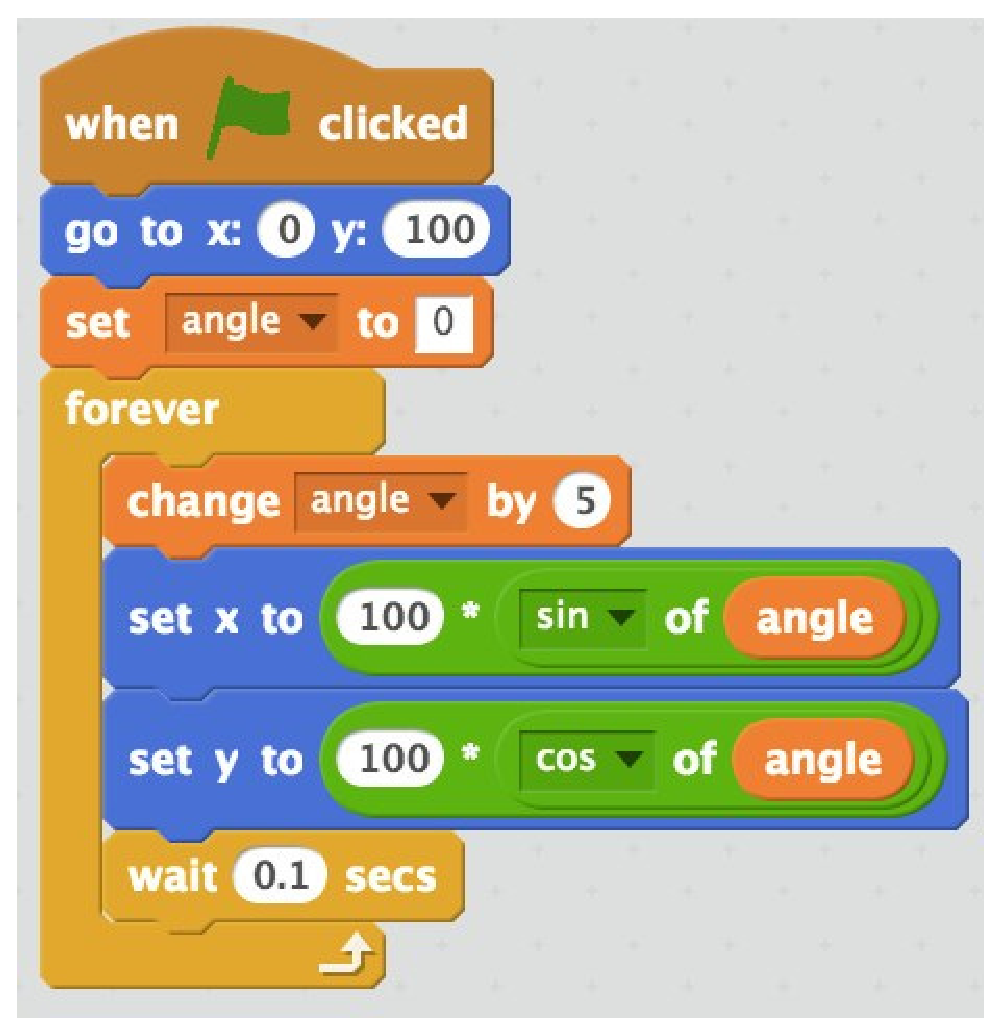
\includegraphics[width=0.5\textwidth]{figuras/scratch_ex1.eps}
    \caption{Exemplo de programa construido por blocos com Scratch. Fonte: Scratch 2.0}
    \label{fig:scratchex1}
\end{figure}

\begin{figure}[H]
    \centering
    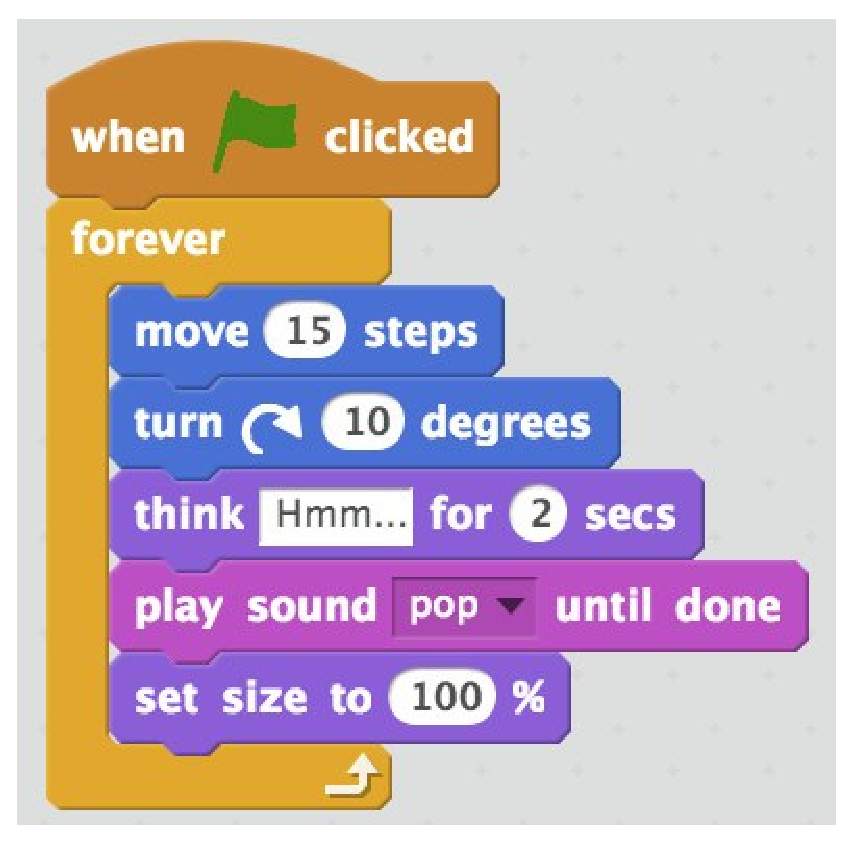
\includegraphics[width=0.5\textwidth]{figuras/scratch_ex2.eps}
    \caption{Exemplo de programa construido por blocos com Scratch. Fonte: Scratch 2.0}
    \label{fig:scratchex2}
\end{figure}
